Ordena los prismas rectos de menor a mayor volumen. La imagen muestra las bases de los cuerpos.
\begin{center}
    \dashedbox{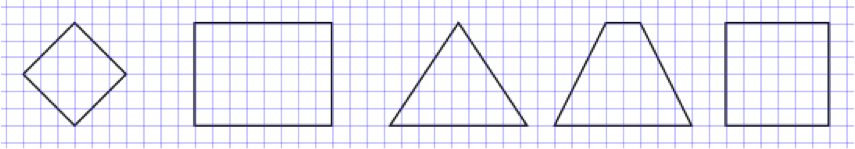
\includegraphics[width=0.8\textwidth ]{../images/sinma2_aiu3_ac80_img08}}
\end{center}
\begin{itemize}
    \item[\rule{1cm}{0.2mm}] 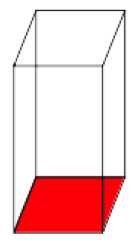
\includegraphics[width=0.05\textwidth ]{../images/sinma2_aiu3_ac80_img13}
    \item[\rule{1cm}{0.2mm}] 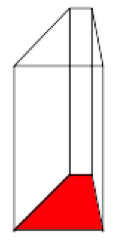
\includegraphics[width=0.05\textwidth ]{../images/sinma2_aiu3_ac80_img11}
    \item[\rule{1cm}{0.2mm}] 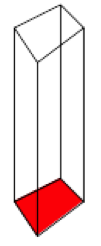
\includegraphics[width=0.05\textwidth ]{../images/sinma2_aiu3_ac80_img09}
    \item[\rule{1cm}{0.2mm}] 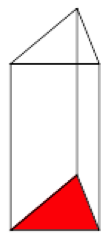
\includegraphics[width=0.05\textwidth ]{../images/sinma2_aiu3_ac80_img10}
    \item[\rule{1cm}{0.2mm}] 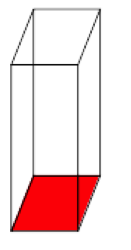
\includegraphics[width=0.05\textwidth ]{../images/sinma2_aiu3_ac80_img12}
\end{itemize}